\chapter{Anhang}
%
\begin{table}[ht]
    \centering
    \caption[Messung lange Spule]{Messwerte Teil 1: Lange Spule (\(L=\SI{0,615}{m}\))}
    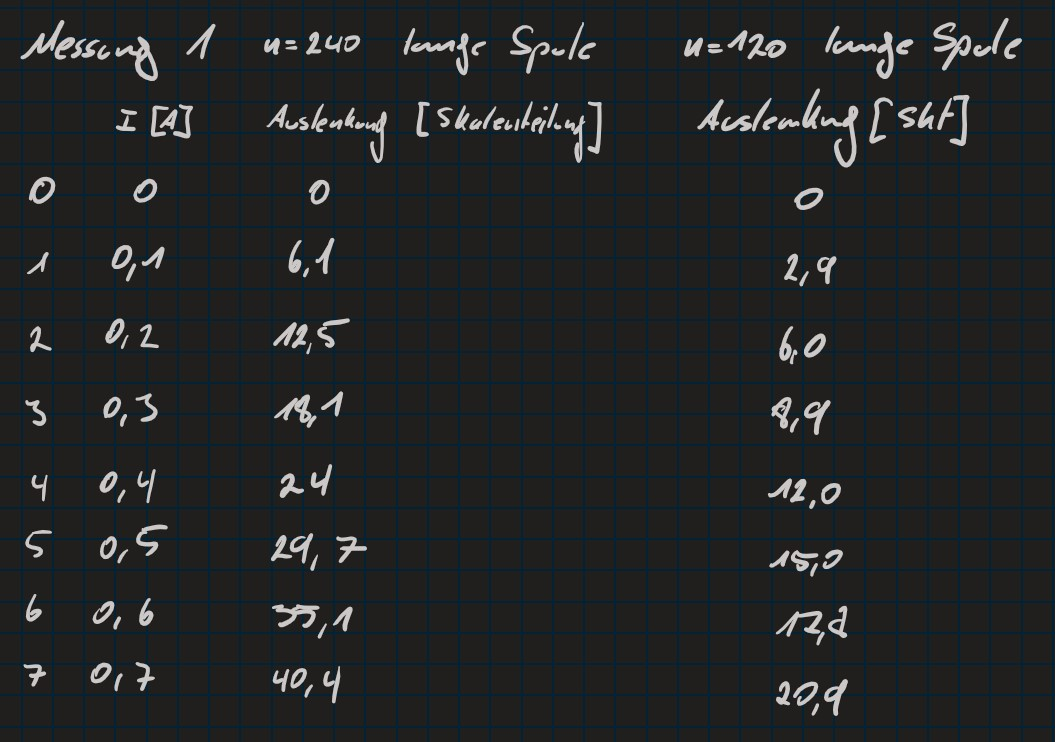
\includegraphics[width=.8\textwidth]{messungen/messung1.jpg}
    \label{tab:mess1}
\end{table}
%
\begin{table}[ht]
    \centering
    \caption[Messung kurze Spule \(D=\SI{0,2}{m}\)]{Messwerte Teil 2: Kurze Spule (\(D=\SI{0,2}{m}\))}
    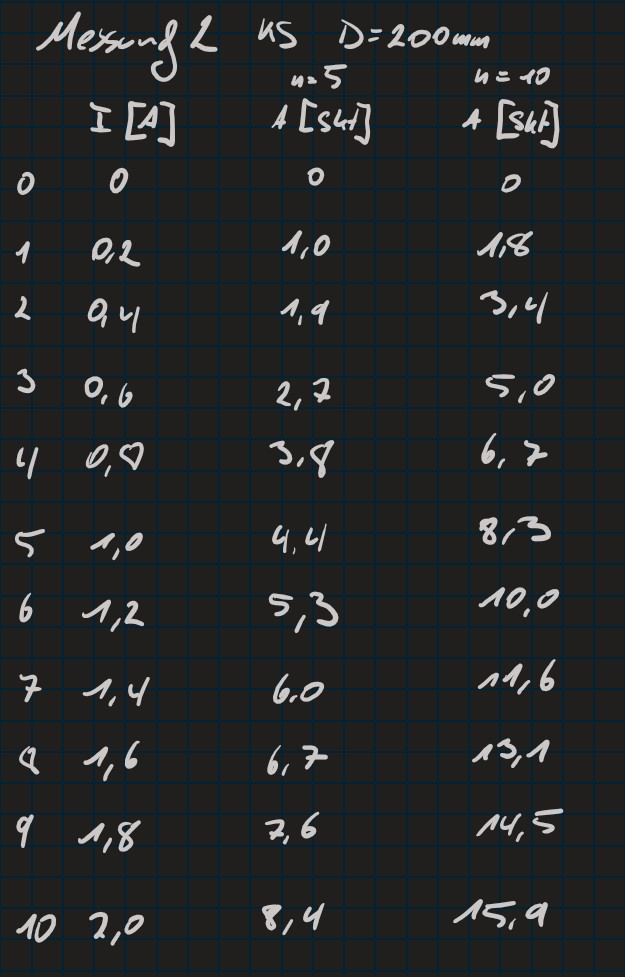
\includegraphics[height=.75\textheight]{messungen/messung2.jpg}
    \label{tab:mess2}
\end{table}
%
\begin{table}[ht]
    \centering
    \caption[Messung kurze Spule \(D=\SI{0,4}{m}\)]{Messwerte Teil 3: Kurze Spule (\(D=\SI{0,4}{m}\))}
    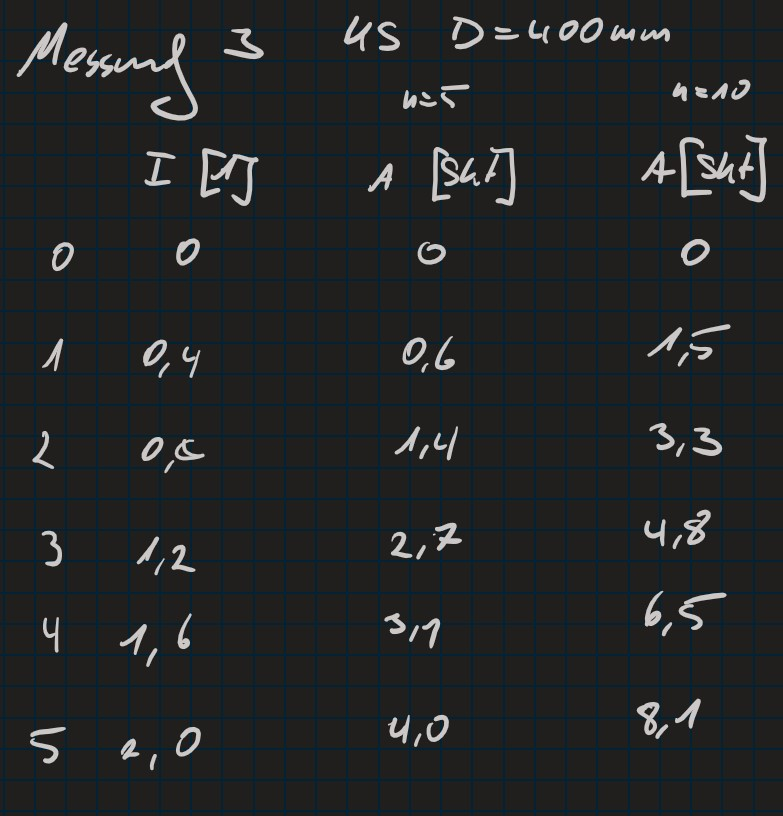
\includegraphics[height=.5\textheight]{messungen/messung3.jpg}
    \label{tab:mess3}
\end{table}